\documentclass[conference]{IEEEtran}
\IEEEoverridecommandlockouts
\usepackage{cvpr}
\usepackage{times}
\usepackage{epsfig}
\usepackage{graphicx}
\usepackage{amsmath}
\usepackage{amssymb}

\usepackage{cite}
\usepackage{amsmath,amssymb,amsfonts}
\usepackage{algorithmicx}
\usepackage{graphicx, algorithm, algpseudocode}
\usepackage{textcomp, makecell}
\usepackage{xcolor}


% Include other packages here, before hyperref.

% If you comment hyperref and then uncomment it, you should delete
% egpaper.aux before re-running latex.  (Or just hit 'q' on the first latex
% run, let it finish, and you should be clear).
\usepackage[pagebackref=true,breaklinks=true,letterpaper=true,colorlinks,bookmarks=false]{hyperref}

% \cvprfinalcopy % *** Uncomment this line for the final submission

\def\cvprPaperID{****} % *** Enter the CVPR Paper ID here
\def\httilde{\mbox{\tt\raisebox{-.5ex}{\symbol{126}}}}

% Pages are numbered in submission mode, and unnumbered in camera-ready
\ifcvprfinal\pagestyle{empty}\fi
\begin{document}

%%%%%%%%% TITLE
\title{The Decision Making of Autonomous Vehicles: A Survey}

\author{Wenxing Lan\\
Department of Computer Science and Engineering\\
Southern University of Science and Technology, Shenzhen, China.\\
{\tt\small 12032882@mail.sustech.edu.cn}
% For a paper whose authors are all at the same institution,
% omit the following lines up until the closing ``}''.
% Additional authors and addresses can be added with ``\and'',
% just like the second author.
% To save space, use either the email address or home page, not both

}

\maketitle
%\thispagestyle{empty}

%%%%%%%%% ABSTRACT

\begin{abstract}
	Autonomous driving is an immature technology, but it can improve the safety, efficiency and convenience of automobile transportation. Therefore, it has great research significance. This paper investigates the decision-making system in the architecture of the autonomous driving system of autonomous vehicles. Decision-making systems are usually divided into many subsystems, which are responsible for tasks such as route planning, route planning, behavior selection, motion planning. In this survey, we have introduced every subsystem in the decision-making system. Finally, the future research directions and applications of decision-making systems are outlined.
\end{abstract}

\begin{IEEEkeywords}
	Autunomous vehicle, decision making, route planning, path planning, behavior selection, motion planning
\end{IEEEkeywords}

\section{Introduction}
Autonomous vehicles (also known as self-driving vehicles and driverless vehicles) have been researched by many universities, research institutes, internet companies, vehicle companies and companies of other industries around the world since the middle 1980s~\cite{self_driving}. In the last two decades, several crucial of autonomous vehicle research platforms are as follows: the Navlab's mobile platform~\cite{Thorpe199144}, University of Pavia's and ARGO, Parma's vehicle~\cite{Broggi199955}, and VaMoRs and VaMP which are autonomous vehicles of UBM~\cite{Gregor200248}.

In the last decade, the Defence Advanced Research Projects Agency (DARPA) held three competitions to accelerate the development of correlation technique about autonomous vehicles~\cite{Brian2016}. In 2004, the first competition named as DARPA Grand Challenge was held in the Mojave Desert, USA~\cite{self_driving}. The goal is to get autonomous vehicles to travel 140 miles of off-road routes as fast as possible~\cite{Brian2016}. Unfortunately, there is no autonomous vehicle which was able to complete the whole journey~\cite{self_driving}.

In 2005, the DARPA Grand Challenge was held again and required autonomous vehicles to travel 132 miles of difficult desert roads across Nevada which contain a mixture of featureless terrain, dust, global positioning system drop-outs, narrow openings, railroad overpasses, bridges, long tunnels, sharp turns, obstacles and a narrow winding mountains road with a 200-foot drop-off~\cite{Buehler2007}. This competition had 23 finalists and 4 cars finished the course within 10-hour limit. Remarkably, the Stanford University's vehicles, Stanley, won the first-place prize, and the Carnegie Mellon University's cars, Sandstorm and H1ghlander, came in second and third place, respectively~\cite{Buehler2007}.

The third competition which is named as the DARPA Urban Challenge was held at the now-closed George Air Force Base, California, USA, in 2007. The objective was for a autonomous vehicles to complete the 60 mile course in less than 6 hours. Additionally, the autonomous vehicles were asked to obey all traffic regulations which avoiding other vehicles including driverless and humandriven vehicles~\cite{buehler2009darpa}. There are 11 finalists in this competition and 6 vehicles completed the route within the allotted time limit. Specifically, Boss, the vehicle of Carnegie Mellon University, won the first-place prize, the Stanford University's vehicle, Junior, claimed second place, and the Virginia Tech's car, Odin, finished in third~\cite{buehler2009darpa}. Although the challenges presented by these competitions cannot cover all the challenges encountered in everyday traffic, they have been hailed as milestones in the development of autonomous vehicles~\cite{Brian2016}.

After the DARPA Challenge, there was a flood of driverless events. Relevant examples include: Intelligent Vehicle Future Challenges~\cite{xin2014china}, from 2009 to 2013; Hyundai Autonomous Challenge~\cite{Cerri2011}, which was held in 2010; VisLab Intercontinental Autonomous Challenge~\cite{broggi2012vislab}, in 2010; the Grand Cooperative Driving Challenge (GCDC)~\cite{Englund2016}, in 2011 and 2016 and Public Road Urban Driverless-Car Test~\cite{Broggi2015}, which was held in 2013. At the same time, many industrial and academic teams have invested a lot of research and development energy in the field of autonomous driving. Among them, the industry is represented by the OEMs of Ford, Toyota, Hyundai and other car companies, as well as IT and emerging companies such as Waymo, Tesla, Uber, Intel, Baidu, Pony.ai, etc., and have developed various autonomous vehicle platforms based on commercialization goals; Academia, including CMU, Stanford, UC Berkeley, Tsinghua University, Tongji University, Southern University of Science and Technology and other major domestic and foreign universities have carried out a series of researches around the key technical fields of autonomous driving.

In order to regulate the application of unmanned driving technology, the National Highway Transportation Safety Administration of the United States Department of Transportation has divided the level of automatic driving (based on the SAE International Standard J3016~\cite{sae2018taxonomy}):
\begin{enumerate}
	\item Level 0 (manual driving): completely controlled by a human driver;
	\item Level 1 (assisted driving): The driving environment provides support for acceleration,  one of the steering wheel and deceleration operations, and the rest is operated by humans. Contains basic auxiliary driving, such as adaptive electronic stability control system (ESC), anti-lock brake system (ABS) and cruise control (ACC);
	\item Level 2 (semi-automatic driving): The driving environment provides support for multiple operations in the steering wheel and acceleration and deceleration, and the rest is operated by humans.  Contains some advanced auxiliary driving functions, such as a horizontal/vertical control system with minimal risk, emergency braking, etc.;
	\item Level 3 (Highly Autonomous Driving): The unmanned driving system completes all operations, but requires the human driver to take over when leaving the operational scene of unmanned driving.
	\item Level 4 (Ultra-high auto-driving): An unmanned driving system with limited roads and environmental conditions, and does not require human drivers to respond to system requests.
	\item Level 5 (Fully Automated Driving): Unmanned driving system that does not limit roads and environmental conditions
\end{enumerate}

The perception system and the decision-making system are two main parts of the autonomy system architecture of autonomous vehicle~\cite{Brian2016}. To limit the range of this survey, We focus on some aspects of decision-making system, which includes route planning, path planning, behavior selection, motion planning, obstacle avoidance, in particular, suitable for systems with automation level 3 or higher~\cite{self_driving}.
The remainder of the paper id structured as follows:
\begin{enumerate}
	\item Overview of the Decision-Making Hierarchy
	\item Route planning
	\item Path planning
	\item Behavior selector
	\item Motion planning
	\item Obstacle Avoidance and control
	\item Conclusion
\end{enumerate}


\section{Introduction of the Decision-Making System}

\begin{figure}[htbp]
	\centering
	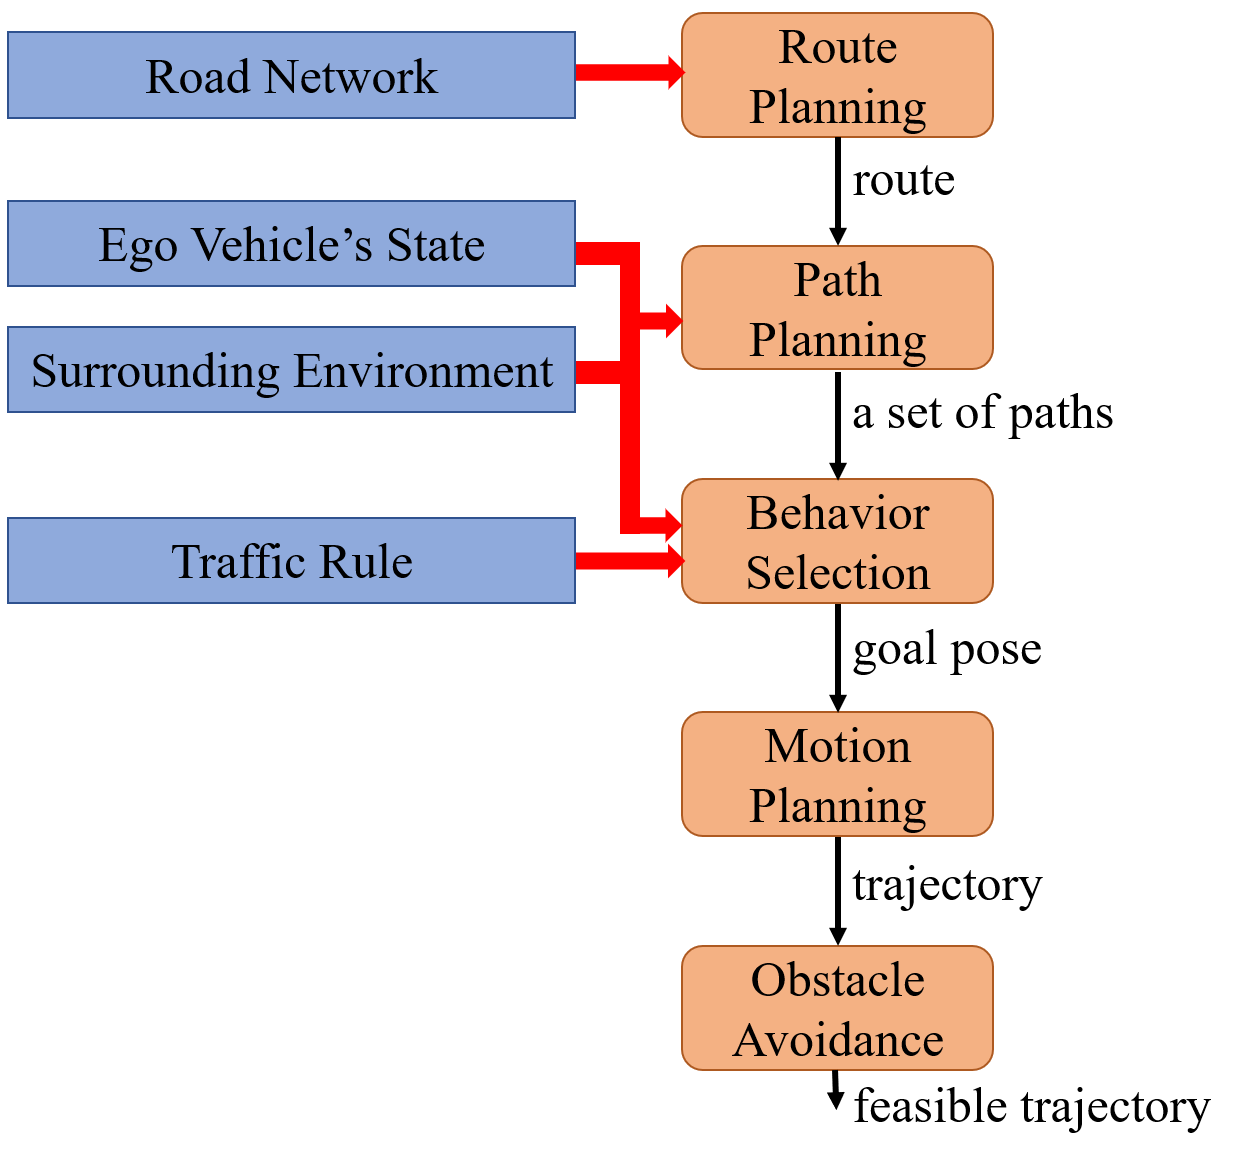
\includegraphics[width=1\columnwidth]{./picture/architecture.png}
	\caption{\label{architecture}
		The five subsystems of decision making system of a typical autonomous vehicle.}
\end{figure}

In this section, the decision making system of a typical autonomous vehicles is described and the brief description of each component of decision making system is provided. The perception system of autonomous vehicles use data captured by on-board sensors, such as Light Detection and Ranging (LIDAR), Global Positioning System (GPS), camera, Inertial Measurement Unit (IMU), Radio Detection and Ranging (RADAR), odometer, etc., and prior information about the models of sensors, road network, traffic rules, vehicle dynamics, etc. to estimate the state of vehicles and create representation of the surrounding environment~\cite{self_driving}. Then, the decision making system use the estimation and environment constructed to control the vehicle in order to reach the goal object~\cite{Brian2016}. 

There are six subsystems which are shown as the orange blocks in Fig~\ref{architecture} in the decision making system of a typical autonomous vehicles~\cite{self_driving}. The brief description of each subsystem is shown as belows.

\subsection{Route Planning Subsystem}
Given a requested destination defined in the road network by the user, the route planning subsystem aims to compute a route, $R$, through the road network from its current position to the requested destination~\cite{Brian2016}. A route, $R=\{r_1, r_2,...,r_{|R|}\}$, is a sequence of way point, where each way point, $r_i$ where $i \in \{1,2,...,|R|\}$, is a coordinate pair. i.e. $r_i = (x_i, y_i)$, in the road network~\cite{self_driving}. Actually, route palnning is a kind of global route planning since it needs to find the complete route from ego vehicle's current position to the final goal, such as the route planned by the BAIDU maps\footnote{https://map.baidu.com/}. The related methods for route planning is shown is Section~\ref{sec:route_planner}.

\subsection{Path Planning Subsystem}
Given a route computed by the route planning subsystem, the path planning subsystem computes a set of paths, $P=\{B_1, B_2, ..., B_{|B|}\}$ by considering the ego vehicle's current state and the traffic rules as well as the surrounding environment~\cite{self_driving}. A path is a sequence of poses, i.e. $B_j=\{b_1, b_2, ..., b_{|B_j|}\}$ where $j \in \{1, 2,...,|P|\}$~\cite{self_driving}. Additionally, each pose, $p_i$, is a coordinate tuple in the static map which only has static object, such as static obstacles, buildings and roads, aroung the ego vehicle and the desired vehicle's orientation at the position defined by this tuple, i.e., $b_i=(x_i, y_i, \theta_i)$~\cite{self_driving}. The relevant methods used in path planning subsystem will be given in Section~\ref{sec:path_planner}.

\subsection{Behavior Selection Subsystem}
The behavior selection subsystem is responsible to select the current reasonable driving behavior for the vehicle according to the behavior, traffic rules and road conditions of the current surrounding traffic participants~\cite{Brian2016}. The behaviors output here are specific driving maneuvers, such as acceleration and deceleration, lane change, overtaking, and following~\cite{Brian2016}. Additionally, the behavior selection subsystem need to select a pose in a selecting path among a set of paths generated by path palnning subsystem a few seconds ahead of the current ego vehicle's state~\cite{self_driving}. The relevant methods used in Path Behavior Selector is shown in Section~\ref{sec:behavior_selector}.

\subsection{Motion Planning Subsystem}
When the behavior is selected by the behavior selection subsystem (for example, it may be lane changing or left turning), motion planning subsystem needs to find a trajectory $T$ which is form the current ego vehicle's state to the curent goal state~\cite{Brian2016}. More importantly, the trajectory needs to satisfy the kinematic and dynamic constraints and be confortable for passengers~\cite{self_driving}. The trajectory $T=\{d_1, d_2, ..., d_{|T|}\}$ can be defined as a sequence of commands, $d_k=(v_k, \phi_k, \Delta_{t_k})$, where $v_k$ denotes the desired velocity at time $k$, $\phi_k$ represents the desired steering angle at time $k$, and $\Delta_{t_k}$ is the duration of $d_k$~\cite{self_driving}. In Section~\ref{sec:motion_planner}, the detail of methods used in motion planning subsystem will be given.

\subsection{Obstacle Avoidance Subsystem}
The obstacle avoidance subsytem needs to change the trajectory (usually decreasing the speed) which is the output of motion planning subsystem in order to avoid collision with other obstacle~\cite{self_driving}.  There is little literature on how to perform the function of this subsystem. Some of the literature related to this subsystem will be discussed in Section~\ref{sec:obstacle_avoider}.


\section{Related Work of Route Planning Subsystem}\label{sec:route_planner}
In this section, the related techniques reported in the literature for the Route Planning subsystem will be surveyed.

The road network, which is the input of the route planning subsystem, is usually represented as a weighted directed graph $G=(V, E)$~\cite{self_driving}. As a assumption, the weight of each edge is always a nonnegative value. In weighted directed graph $G$, each vertex $v_i$ where $v_i \in V=\{v_1, v_2, ..., v_{|V|}\}$ is road junction, such as crossroads, three forks, etc., and each directed edge $e_{ij}$ where $e_{i,j} \in E, i \neq j$ connects pairs of road junctions $v_i$ and $v_j$. Specifically, edge weight $w_{ij}$ denotes the cost of traversing edge $e_{ij}$. Computing a route, the task of route planning subsystem, can be reduced to find a path in a weighted directed graph. Normally, the path should be shorest since most users are willing to reach destination as soon as possible~\cite{self_driving}. Unfortunately, classical shortest path algorithms, such as Dijkstra~\cite{dijkstra1959note} and $A^*$~\cite{Hart1968formal} are impractical because of their high time complexity to large road networks, such as city road network or even nation road network~\cite{self_driving}.

The performance of route planning algorithms in road networks has improved significantly in the past decade~\cite{self_driving}. The driving direction can be calculated by some newly developed algorithm in milliseconds or less, even at national scale~\cite{bast2016route}. Various technologies supply different balance between preprocessing effort, query time and space usage~\cite{bast2016route}. The queries can be responded in less than a microsecond by some alforihtms, while the real-time traffic can be effectively handled by other algorithm~\cite{bast2016route}. The techniques used in route planning in a road network can be divided into six classes~\cite{bast2016route}:
\begin{enumerate}
	\item Basic Techniques
	\item Goal-directed Techniques
	\item Separator-based Techniques
	\item Hierachical Techniques
\end{enumerate}

\subsection{Basic Techniques}\label{subsec:basic_techniques}
Dijkstra's algorithm provides a standard solution to the one-to-all shortest path problem in a weighted directed graph, and pesudo code of Dijkstra's algorithm is shown in Algorithm~\ref{dijkstra}~\cite{dijkstra1959note}. \emph{label-setting}, one of the property of Dijkstra's algorithm, means that the traversing cost from start site $v_s$ to destination site $v_e$ is shortest once the destination site $v_e$ has been scanned~\cite{dijkstra1959note}. Consequently, the algorithm can be stopped as soon as it has been scanned the destination site for one-to-one queries~\cite{bast2016route}. The time complexity of Dijkstra's algorithm is influenced by the using priority queue. For example, the time complexity is $O((|V|+|E|)log|V|)$ if the priority queue is binary heaps~\cite{forsythe1964algorithms}.
\begin{algorithm}[htbp]
	\caption{\label{dijkstra}Dijkstra's Algorithm~\cite{dijkstra1959note}.}
	{\bf Input:} weighted directed graph $G=(V, E)$; start vertex $v_s \in V$
	\begin{algorithmic}[1]
		\State Initial a priority queue $Q=\{v_s\}$ of vertices which is ordered by total traversing cost from $v_s$.
		\State Initial all traversing cost $cost(v_s, v_i)=+\infty$ where $v_i \in V$.
		\State Set $cost(v_s, v_s) = 0$.
		\While {not all vertex $v \in V$ has been traversed}
		\State Exact a vertex $u$ with minimum traversing cost from $Q$.
		\State Find all arcs $E' = \{e | e=(u, v) \in E\}$ incident to $u$.
		\For {each $e=(u,v) \in E'$}
		\If {$cost(v_s, u)+w(u,v) < cost(v_s, v)$}
		\State Set $cost(v_s, v) = cost(v_s, u)+w(u,v)$.
		\EndIf
		\State Add $u$ into $Q$.
		\EndFor
		
		\EndWhile
		\State Return all traversing cost.
	\end{algorithmic}
\end{algorithm}

Bellman-Ford algorithm is an alternative method which can compute shortest path in a weighted directed graph~\cite{bellman1958routing, ford1956network}. At each iteration, it scans all vertices whose traversing cost have improve~\cite{bellman1958routing, ford1956network}. It often uses a simple FIFO queue to keep track of vertices to scan next~\cite{bast2016route}.  Additionally, Bellman-Ford algorithm has the \emph{label-correcting} property: each vertex may be scanned many times, and the time complexity of this algorithm is $O(|V||E|)$. Finally, the Floyd-Warshall algorithm calculates traversing cost between all pairs of vertices in $O(|V|^3)$ time~\cite{floyd1962algorithm}. It is more suitable for sufficiently dense graphs than Dijkstra's algorithm~\cite{bast2016route}.

In summary, these algorithm metioned above are the basic algorithm to find shortest path in a weighted directed graph. Although they all have high time complexity, they always can find one shortest path in a given nonegative weighted directed graph.

\subsection{Goal-directed Techniques}
By avoiding scanning the vertices that are not in the direction of the target vertex, the goal-directed technology guides the search from the source vertex to the target vertex~\cite{bast2016route}.

$A^*$ algorithm, a classic goal-directed shortest path algorithm, uses a heuristic function $f(u,t)$ to estimate the traversing cost from vertex $u$ to $t$ ($t$ is usually the destination site.)~\cite{Hart1968formal}. Normally, the value of $f(u,t)$ is the lower bound of the traversing cost from vertex $u$ to $t$. Then, it runs a modified version of Dijkstra's algorithm which regards the value computed by the formula $cost(v_s, u)+f(u,t)$ as the prioirty of a vertex $u$~\cite{bast2016route}. Therefore, the vertices which are much closer to the destiniation site $t$ will be scanned earier during the implementation of the algorithm~\cite{bast2016route}. ALT ($A^*$, landmarks, and triangle inequality) algorithm uses inequality property among landmarks to automatically obtain a heuristic function with better lower bounds in order to replace the user-defined heuric function in $A^*$ algorithm~\cite{goldberg2005computing}. 

Arc flags, an another goal-directed method, needs to divide the grah into $C$ cells which are roughly balanced (have similar number of vertices) and have a few boundary vertices during preprocessing~\cite{hilger2009fast, lauther2006experimental}. A vertoc of $C$ bits, named as arc flags, is maintained by each arc~\cite{hilger2009fast, lauther2006experimental}. Additionally, if the arc lies on a shortest path to some vertex of cell $i$, the $i$-th bit is set~\cite{hilger2009fast, lauther2006experimental}. The arc marking of unit $i$ is calculated by growing the shortest path tree backward from each boundary vertex and setting the $i$-th flag for all arcs (i.e. edges) of the tree~\cite{hilger2009fast, lauther2006experimental}. In the query phase, the algorithm prunes the arcs that are not labeled for the pixels that contain the target vertices~\cite{bast2016route}. The preprocessing time of arc flags algorithm is high, but the query time of arc flags algorithm is the fastest among goal-directed technology~\cite{self_driving}.

In summary, these algorithms mentioned above use destination site as information to guide search process. Therefore, the search process is more targeted. Additionally, all of them use heuristic function which is user-defined or obtained by structure of the graph to estimate the cost between experted exploring vertex and destination vertex.

\subsection{Separator-based Techniques}

Either vertex or arc is regarded as separator of graph among the methods using separator-based techniques~\cite{self_driving}. The vertex (or arc) separator is a small part of a vertex (or arc), and its removal breaks the graph into several balanced components~\cite{bast2016route}. The algorithm based on vertex separator uses vertex separator to calculate overlay~\cite{bast2016route}. Quick arcs are added to the overlay to preserve the distance from any pair of vertices in the entire graph. The overlay graph is much smaller than the complete graph and is used to speed up the query algorithm~\cite{bast2016route}. High performance multi-level routing (HPML) algorithm is a variant of this method~\cite{delling2009high}. It significantly reduces query time by adding more shortcuts to the graph, but spans different levels at the cost of increasing space usage and preprocessing time~\cite{delling2009high}.

The algorithm based on arc separator reduces the number of cutting arcs connecting the boundary vertices of different elements as much as possible~\cite{bast2016route}. In order to preserve the distance between boundary vertices in each pixel, a shortcut is added to the overlay~\cite{bast2016route}. The customized route planning (CRP) algorithm is a variant of this method, which is mainly used to meet the needs of real-world road network, such as dealing with turning costs and performing fast updating of cost functions~\cite{delling2017customizable}. Its preprocessing is divided into two stages~\cite{delling2017customizable}. In the first stage, the superimposed multi-layer partition and topology are calculated~\cite{delling2017customizable}. In the second stage, the cost of group arc is calculated by bottom-up and parallel processing units~\cite{delling2017customizable}.

\subsection{Hierachical Techniques}

The hierarchical method mainly uses the inherent level of road network~\cite{bast2016route}. In the road network, important roads (such as highways) constitute a small arterial subnet. When the query algorithm is far away from the source and target, the algorithm only scans the vertices of the above subnets~\cite{bast2016route}. In the preprocessing stage, the importance of the vertex or arc is calculated according to the actual shortest path structure. The contraction hierarchy (CH) algorithm is a hierarchical technique~\cite{geisberger2012exact}. The main idea is to create a shortcut to skip the less important vertices~\cite{geisberger2012exact}. If the shortest path between them is unique and contains vertices to delete (i.e., shrink), it repeats the vertex shrink operation, which removes the least important vertices from the drawing and creates a shortcut between each pair of adjacent vertices~\cite{geisberger2012exact}. CH can be used as the basis for other point-to-point algorithms and extended queries because it is universal~\cite{geisberger2012exact}.


\section{Related Work of Path Planning Subsystem}\label{sec:path_planner}
In this section, the related techniques reported in the literature for the Route Planning subsystem will be surveyed.

A set of paths, $P=\{B_1, B_2,..., B_{|P|}\}$, are computed by the path planning subsytem by thinking about the route planned by route planning subsystem, the ego vehicle's state, traffic rules and the surrounding environment~\cite{self_driving}. A sequence of pose $p_i=(x_i, y_i, \theta_i)$ makes up a path $B_j=\{b_1, b_2, ..., b_{|B_j|}\}$, and the pose includes the position of vehicle and its orientation in the map~\cite{self_driving}. Algorithms for path planning susbsytem mainly includes two classes: graph serach based and interpolating curve based~\cite{self_driving}.

\subsection{Graph Search Based Algorithms}
In graph search based algorithms, all possible ego vehicle's state make up a state space which is denoted as a graph~\cite{gonzalez2015review}. The best path between ego vehicle's current state and a goal state is searched by this kind of algorithms. Additionally, the goal state is a pose of a way point $w_i$ of the route $W$ obtained by the route planning sussystem~\cite{gonzalez2015review}. For path planning subsystem, Dijkstra, $A^*$ and the variants of $A^*$ are three kinds of most common grap search based algorithms~\cite{self_driving}.

The detail of Dijkstra algorithm can be refered in Section~\ref{subsec:basic_techniques}. Odin, an autonomous vehicel, uses Dijkstra algorithm to compute a path which is entering or away park~\cite{bacha2008odin}. Additionally, Dijkstra algorithm is employed to construct a path in simulation environment~\cite{kala2013multi}. \cite{arnay2016safe} computes a path for the autonomous vehicle Verdino bu using Dijkstra algorithm.

The detail of $A^*$ algorithm can be refered in Section~\ref{subsec:basic_techniques}. Rocky, an autonomous vehicle, computes path with $A^*$ algorithm in the 2005 DARPA Grand Challenge~\cite{Leedy2007}. $A^*$ with two different heuristic cost function is applied to build a path and was tested in an autonomous vehicle, AnnieWAY~\cite{Ziegler2008787}. One heuristic cost function, named as Rotation Translation Rotation (RTR), thinks about the vehicle's kinematics constraints of the car, and the other uses the information of positions and shapes of all obstacles including static obstacles and dynamic obstacles~\cite{Ziegler2008787}.

Other literatures use $A^*$ variants in path planning susbsytem. The anytime $D^*$ is proposed to compute a path for the autonomous vehicles Boss~\cite{Urmson2008}. For the autonomous vehicle Junior, the hybrid-state-$A^*$ is used to construct a path~\cite{Dmitri2010path}. A kind of $A^*$ variant is introduced to generate a smooth path by thinking about the kinematic constraints of vehicles~\cite{chu2015real}.

\subsection{Interpolating Curve Based Algorithms}
Interpolating curve based algorithms insert some new points into a already known set of points (for example, the way points generated by route planning subsystem) to generate a smooth path~\cite{self_driving}. Spline curves are the most used in interpolating curve based algorithms in path planning subsystem~\cite{self_driving}. Cubic spline curve is employed in \cite{chu2012local} and \cite{HU2018482} in path planning subsystem. Both of them build a centerline from the route extracted from the road network~\cite{chu2012local, HU2018482}. They use arc length and offset to the centerline to generate a series of parametric cubic splines that represent possible candidate paths~\cite{chu2012local, HU2018482}. The best path is selected based on the function of safety and comfort~\cite{chu2012local, HU2018482}.

\section{Related Work of Behavior Selection Subsystem}\label{sec:behavior_selector}
In this section, the related techniques reported in the literature for the behavior selection subsystem will be surveyed.

Given a path planned by the path planning subsystem, the behavior selection subsystem needs to select an suitable behavior at any time according to real-time traffic, the behaviors of other traffic participants, traffic rule and traffic signals~\cite{Brian2016}. For example, when a vehicle is approaching an intersection, the behavior layer will command the vehicle when to go straight, turn left or turn right. Methods for behavior selection subsystem can be mainly divided into three classes: finite state machine (FSM) based methods, ontology-based methods and Markov decision processes based method~\cite{self_driving}.

\subsection{FSM-based Methods}
In FSM-based methods, next action of the ego vehicle is selected according to a rule-based decision process in different traffic sence~\cite{self_driving}. Normally, state denotes the behavior and transition conditions are the information extracted from perception system~\cite{self_driving}. The main disadvantage of this method is that it is difficult to model all the uncertain and complex urban traffic scenes~\cite{self_driving}. Junior team used FSM to record several simple urban traffic sences in DARPA Urban Challenge~\cite{buehler2009darpa}. Additionally, the autonomous vehicle A1 used a FSM that had states for more complex traffic scenario to select a suitable driving behavior~\cite{jo2015development}.

Each traffic sence uses a FSM in the IARA's behavior selection subsystem~\cite{guidolini2018handling}. Some state transition rules are checked in order to find next suitable driving behavior in FSM for each scene according to the information provided by perception system~\cite{guidolini2018handling}. A network which mixes decision tree and deterministic automate is a kind of model of the behavior selection subsystem~\cite{Aeberhard2015}. It is a good idea to reduce the model complexity that dividing the driving task into a finite set of logitudinal and laterral guidance states~\cite{Aeberhard2015}. Cruise controls states and a single critical control state are two components of the longitudinal states. The lateral guidance state mainly includes the state about lane keeping or lane chnaging~\cite{Aeberhard2015}. In roundabouts situations, Okumura et al. modeled a high-level behavior selection subsystem as a classifier of hybrid a support vector machine (SVM) and FSM~\cite{Okumura2016}. There are two levels in this behavior selection subsystem~\cite{Okumura2016}. Firstly, the SVM classifier maps the ego vehicle's current state and information provided by perception system to next action of the vehicle~\cite{Okumura2016}. Secondly, the action is tranfer to high-level commands by the FSM~\cite{Okumura2016}. A hierarchical concurrent state machine is used in behavior selection subsystem to due with more complex traffic scenes~\cite{Ziegler2014}. A set of constraints are genrated by this kind of behavior selection subsystem by thinking about information such as lane characteristics~\cite{Ziegler2014}. 

\subsection{Ontology-based Methods}
The ontology that can be used to model concepts and their relationships is a framework for knowledge representation. Modeling of traffic laws and sensor data can use ontology-based knowledge base to help autopilot understand the world~\cite {Zhao2015ontology}. In order to establish the behavior selection subsystem, humans have built a knowledge base based on ontology. Things that happen at intersections and narrow roads are concentrated in ~\cite {Zhao2015ontology}. Rules such as right of way rules are used by the system to consider to make decisions, and decisions such as "stop" or "give way" are sent to the path planning subsystem to change the route or stop to avoid collisions~\cite{Zhao2015ontology}. The disadvantage of this method is that you need to design an accurate world model. Items such as lanes and traffic rules drawn at each location make up the model. These items are usually done manually\ cite {Zhao2015ontology}. In recent work, others have improved previous work so that only a small part of the knowledge base is needed\cite {Zhao20171425}.

\subsection{Markov Decision Processes Based Methods}
The uncertainty in perception and actions transition between states can be solved by the partially observable Markov decision process (POMDP)~\cite{self_driving}. Online POMDP is employed in behavior selection subsystem to change lane in city environments~\cite{Ulbrich2013}. The proposed method is divided into two parts in order to do real-time decision making and reduce the complexity of the POMDP~\cite{Ulbrich2013}. At first, a signal processing network is used to evaluated the situation~\cite{Ulbrich2013}. The network is a graph that thinks about velocities, relative distance and time to collisions with obstacle near the ego vehicle, and output if changing lane or not~\cite{Ulbrich2013}. The POMDP only plans online for the curretn state by using the network output~\cite{Ulbrich2013}.

In order to reson about observation uncertainty and potentially hidden objects, a continuous POMDP method is used by thinking about the interactions of other traffic participants~\cite{Brechtel2014392}. The planning is speeded up by assuming finite number of policies~\cite{Brechtel2014392}. As a first step, the reward function aims to optimize comfort and efficiency by returning the acceleration and deceleration costs to reach the target area~\cite{Brechtel2014392}. This step depends only on the state of the vehicle and the previously defined objectives~\cite{Brechtel2014392}. The second step is to consider other traffic participants by increasing the cost of collision with other road users~\cite{Brechtel2014392}. The reward function is the summation of two steps cost, and the scalar value of it denotes the driving objection~\cite{Brechtel2014392}.

Galceran et al. proposed an integrated reasoning and behavior selection method, which modeled vehicle behavior and nearby vehicles as a group of discrete strategies~\cite{galceran2017multipolicy}. In this work, they used a set of manual design strategies to deal with in lane and intersection driving situations~\cite{galceran2017multipolicy}. In the history of other vehicles, they used Bayesian change point detection to infer possible future actions, thus estimating the distribution of potential strategies that each vehicle in the vicinity might be executing~\cite{galceran2017multipolicy}. Then, the behavior selection algorithm performs the strategy with the maximum reward value by approaching the POMDP solution that evaluates the strategy of the predicted vehicle through forward simulation~\cite{galceran2017multipolicy}. However, they assume that most driving participants follow traffic rules and act in a regular, predictable way. The experiment was carried out on an autopilot vehicle platform~\cite{galceran2017multipolicy}.

Wray proposes an intermodal behavior selection subsystem for automated driving vehicles using interactive multiple online decision components (MODIA) instead of a set of policies~\cite{ijcai2017-664}. Modia models the traffic participants as independent Markov decision process (MDP)~\cite{ijcai2017-664}. Each MDP maintains its own beliefs and proposed actions at each time step, resulting in a set of estimated actions~\cite{ijcai2017-664}. The dictionary performer action function (leaf) performs only the best (in terms of preference) actions in this set (for example, stop actions have preferences)~\cite{ijcai2017-664}. The action can simply stop, edge or walk, and encode the motion by assigning the required velocity and target point along the AV trajectory~\cite{ijcai2017-664}. Modia is still easy to handle because the number of instantiated decision processes increases linearly~\cite{ijcai2017-664}. The method is tested in the automatic driving vehicle under the scene of intersection, and compared with the ignorance and naive baseline algorithm, successfully solving the problem of automatic driving vehicle interaction in the intersection scene~\cite{ijcai2017-664}.

\section{Related Work of Motion Planning Subsystem}\label{sec:motion_planner}
In the autonomous driving system, motion planning is an extremely important module, responsible for generating a safe, effective, and collision-free motion trajectory from the starting point to the destination for the autonomous vehicle~\cite{gonzalez2015review}. In the industry, motion planning is often divided into path planning (global planning) and trajectory planning (local planning)~\cite{gonzalez2015review}. The sequence of points or curves connecting the starting point and the end point is called a path, and the strategy of forming a path is called path planning~\cite{gonzalez2015review}. The goal of path planning is to make the distance between the path and obstacles as far as possible and the length of the path as short as possible; the purpose of trajectory planning is to make the running time of the car as short as possible or the energy as small as possible~\cite{gonzalez2015review}. Trajectory planning adds time series information on the basis of path planning to plan the speed and acceleration of the car when performing tasks to meet the requirements of smoothness and speed controllability~\cite{gonzalez2015review}.

Considering that sometimes the algorithms used in global planning and local planning can be used interchangeably, we will explain the advantages and disadvantages of the methods used in global planning and local planning~\cite{Brian2016}. At present, the more widely used motion planning methods mainly include the following categories: motion planning methods based on graph search, motion planning methods based on random sampling, methods based on numerical optimization, methods based on curve interpolation, methods based on probability, planning methods based on machine learning, etc~\cite{Brian2016}.

\begin{table*}[htbp]
	\centering
	\caption{\label{tab:motion_planning}Pros and Cons of all kinds of Motion planning methods
	}
	\setlength{\tabcolsep}{4pt}
	\begin{tabular}{|c|c|c|}%{|m{1.9cm}|m{7.6cm}|m{7.6cm}|}
		\hline
		\multicolumn{1}{|c|}{\textbf{Algorithm}} & \multicolumn{1}{|c|}{\textbf{Pros}} & \multicolumn{1}{|c|}{\textbf{Cons}} \\
		\hline
		Dijkstra~\cite{dijkstra1959note} & \makecell[l]{1. Suitable for structured or unstructured roads. \\ 2. The shortest path can be found in the grid map.\\}  & \makecell[l]{1. Due to the need to traverse the nodes, the computational cost is large.\\ 2. The path obtained is not continuous and is not suitable for automatic\\ driving scenarios that require real-time calculation.}\\
		\hline
		$A^*$ series~\cite{Hart1968formal} & \makecell[l]{1. Extension of Dijkstra's algorithm. \\ 2. A heuristic algorithm.\\ 3. Can reduce calculation time. \\}  & \makecell[l]{1. The searched path is not continuous.\\ 2. The heuristic rule is not applicable in some scenarios.}\\
		\hline
		Status grid~\cite{Pivtoraiko2005} & \makecell[l]{1. Can handle multi-dimensional issues (such as position,\\ velocity, acceleration, time, etc.). \\ 2. Suitable for local planning in a dynamic environment.\\}  & \makecell[l]{1. Computationally expensive.\\ 2. Only suitable for more discrete state space.}\\
		\hline
		RRT series~\cite{karaman2011sampling} & \makecell[l]{1. Can provide a fast search algorithm in complex space.\\ 2. Both global planning and local planning can be used.\\}  & \makecell[l]{1. The resulting trajectory is not continuous.\\ 2. The optimization degree of the trajectory is more dependent on the\\ time frame sequence of the RRT.}\\
		\hline
		Curve interpolation~\cite{gonzalez2015review} & \makecell[l]{1. Suitable for curve smoothness optimization.\\ 2. Can generate a comfortable and continuous trajectory \\in a dynamic environment.\\ 3. Simple calculation. \\}  & \makecell[l]{1. Rely on the path points generated by the global plan.\\ 2. Large computational expense when dealing with obstacle scenes.}\\
		\hline
		Clothoid~\cite{brezak2013real} & \makecell[l]{1. Smooth transition between straight line and curve.\\ 2. Suitable for local planning.\\}  & \makecell[l]{1. Due to the definition of curve integral, the calculation consumes a lot.\\ 2. The curve is continuous but not smooth}\\
		\hline
		Polynomial curve~\cite{piazzi2002quintic,glaser2010maneuver,simon1999vehicle} & \makecell[l]{1. Low computational cost.\\ 2. Can generate continuous smooth motion trajectory\\}  & \makecell[l]{1. It is often a polynomial of order 4 or higher, resulting in a large \\ computational cost.}\\
		\hline
		Bezier curve~\cite{rastelli2014dynamic, choi2008path} & \makecell[l]{1. Low computational cost. \\2. Curve shape can be determined by control points.\\ 3. Continuous smooth motion trajectory can be generated\\ }  & \makecell[l]{1. Rely on the path points generated by the global plan. \\ 2. When the curve dimension is increased, the calculation consumes \\ more. }\\
		\hline
		Spline curve~\cite{shiller1991dynamic, berglund2009planning} & \makecell[l]{1. Low computational cost.\\ 2. Continuous curve is controlled by different nodes\\ }  & \makecell[l]{1. The resulting path may not be optimal. }\\
		\hline
	\end{tabular}
\end{table*}


\subsection{Graph Search Based Methods}
The basic idea of the method based on graph search is to traverse the space from point A to point B. This method usually represents the state space as an occupancy grid or grid, which describes objects in the environment. From a planning point of view, a path can be set to implement the graph search algorithm to access different states in the grid and provide solutions.  Some of these algorithms have been applied to the development of autonomous vehicles.

Dijkstra algorithm is a graph search algorithm to find the single source shortest path in the graph~\cite{dijkstra1959note}. The configuration space is approximately a discrete unit grid space, lattice, such as~\cite{marchese2006multiple} and \cite{lavalle1998optimal}.  The concept and implementation of the algorithm are described in \cite{lavalle2006planning} and \cite{hwang2003fast}.  In autonomous driving, it has been implemented by \cite{kala2013multi} in a multi-cabin simulation, with the Ben Franklin Racing Team entering the DARPA Urban Challenge \cite{bohren2008little} and Victor Tango Team \cite{bacha2008odin}.

$A^*$ algorithm is a heuristic implementation based on graph search algorithm, enabling fast node search (it is an extension of Dijkstra graph search algorithm)~\cite{Hart1968formal}.  Its most important design aspect is the determination of the cost function, which defines the weight of the node, which is suitable for searching the space mainly known in advance by the vehicle \cite{likhachev2009planning}, but its cost is higher in terms of memory and speed~\cite{Hart1968formal}.

Some path planning algorithms for mobile robots have also been used as improvements, and are used in autonomous driving systems, such as Field D star~\cite{ferguson2006using}, Theta star~\cite{KAHANA2001739}, Anytime repairing A star (ARA star) and anytime D star (AD  star)~\cite{LIKHACHEV20081613} and so on.  Ziegler et al. applied A star algorithm and Voronoi cost function to plan unstructured space application scenarios~\cite{Ziegler2008}.

State grid algorithm uses the discrete of the planned area of the state grid to represent the actual road environment~\cite{self_driving}. This grid is called the status grid~\cite{Brian2016}. The motion planning search is applied in \cite{Pivtoraiko2005}. The path search in this algorithm is based on a set of grids containing all feasible features, allowing the vehicle to travel from the initial state to several other states~\cite{Pivtoraiko2005}. The cost function determines the pre-calculated optimal path grid~\cite{Pivtoraiko2005}.

\subsection{Random Sampling Based Methods}
This type of planning method attempts to solve the problem of time constraints, that is, a type of problem that cannot be satisfied by using deterministic methods in high-dimensional spaces~\cite{Brian2016}. This broad category of methods includes random sampling configuration space or state space, among which the most commonly used methods are the Probabilistic Road Map Method (PRM)~\cite{kavraki1996probabilistic} and the Rapid Exploration Random Tree (RRT)~\cite{lavalle2001randomized}. The latter has a wide range of applications in the field of autonomous driving.

Rapid Search Random Tree (RRT): It is a sampling-based algorithm used in path planning~\cite{karaman2011sampling}. It can perform rapid planning in a semi-structured space~\cite{lavalle2001randomized}, and then perform random search through the navigation area. So as to plan a suitable path~\cite{karaman2011sampling}. This method can also consider some incomplete constraints, such as the maximum turning radius and momentum of the vehicle~\cite{karaman2011sampling}.

These algorithms are reviewed in~\cite{elbanhawi2014sampling} and~\cite{karaman2011sampling}. In the autonomous driving system, this type of algorithm has been used by the MIT team in the DARPA Urban Challenge~\cite{Kuwata2009}.  However, the resulting path is not optimal. In~\cite{karaman2010optimal}, an algorithm named RRT star was developed, which can achieve convergence to the optimal solution.

\subsection{Numerical Optimization Based Methods}
Numerical optimization based methods includes various methods based on numerical optimization and nonlinear optimization. These methods consider the influence of different constraint variables, and then generate the optimal path by minimizing or maximizing the function~\cite{Brian2016}. In the actual path planning method, it usually optimizes the previously rough trajectory to generate a smooth and feasible trajectory~\cite{dolgov2010path}. In addition, the optimal trajectory is also calculated from the kinematics-based constraints~\cite{ziegler2014making}.

Function optimization finds the root of an actual value function (minimize variable result)~\cite{Brian2016}. It can be used to improve the potential field method (PFM) and be applied to mobile robots in narrow passage environments and autonomous vehicles in special situations~\cite{Brian2016}. This type of method can realize continuous trajectory position, velocity, and acceleration as planning parameters~\cite{Brian2016}.

\subsection{Curve Interpolation Based Methods}
The curve used in curve interpolation based methods includes Clothoid curve, polynomial curve, Bezier curve and spline curve method, etc~\cite{Brian2016}. Computer-aided geometric design technology is often used to solve smooth path points for a given path~\cite{brezak2013real}.  This allows the motion planning algorithm to consider its feasibility, comfort, and vehicle dynamics related parameters to generate the required trajectory~\cite{brezak2013real}.

Interpolation is defined as constructing and inserting a set of new data, known set reference points, within the previous data range~\cite{gonzalez2015review}. This means that these algorithms can use the previous set of path points to generate a new set of data (that is, a smoother path), which is more conducive to the continuity of the trajectory and is more suitable for the constraints of vehicle driving and dynamic environment~\cite{gonzalez2015review}. When planning, if there are obstacles, it can generate a new path, and then re-input the previously planned path to get the feasible trajectory we want~\cite{gonzalez2015review}.

The method based on the clothoid curve is defined based on the Fresnel integral~\cite{brezak2013real}. The use of clothoid curves can define the trajectory of linear changes in curvature, because their curvature is equal to the arc length; and smooth transitions can be made between straight and curved segments~\cite{brezak2013real}. This type of method has been applied in highway and railway driving scenarios, and it is also suitable for some wheeled mobile robots~\cite{walton2005controlled}.

Polynomial curves are usually implemented to meet the constraints required by their interpolation points, where the constraints specifically include fitting position, angle, and curvature~\cite{gonzalez2015review}. The expected values or constraints in the beginning and end of this type of method will determine the coefficient of the curve. For the calculation of polynomial coefficients, please refer to~\cite{piazzi2002quintic}, \cite{glaser2010maneuver} and~\cite{simon1999vehicle}.


Bezier curve is a kind of parametric curve method, which relies on control points to determine the curve shape. The core of the Bezier curve is the Bernstein polynomial. This type of method has been widely used in CAGD applications, technical drawing, aviation, and automotive design. Its advantage is low computational cost, because the shape of the curve is determined by the control points. We can place these control points correctly to meet the constraints of the beginning and end of curvature~\cite{rastelli2014dynamic}, \cite{choi2008path}.


A good example of Bezier modularity and ductility is in~\cite{setsompop2012blipped}, which can generate interconnected circular shapes and interconnected Bezier curves with continuous curvature. These curves are usually used to approximate cyclotron curves \cite{wang2001approximation}, \cite{sanchez2003polynomial}, or to achieve reasonable Bezier rapid planning curves, such as spline curve. Spline is a piecewise polynomial parameter in the graded interval~\cite{montes2008real}. The curve is defined as a polynomial curve~\cite{piazzi2002quintic}. In fact, B-spline~\cite{shiller1991dynamic, berglund2009planning} can also be represented by Bezier curve~\cite{elbanhawi2014sampling} or clothoid curve~\cite{walton2005controlled}. The connections between each sub-segment are called knots, and they usually have a high degree of smoothness constraints~\cite{elbanhawi2014sampling, walton2005controlled}.

\subsection{Probability Based Methods}
It mainly includes probability-based planning methods such as MDP and POMDP~\cite{Brian2016}. When dealing with uncertainties in dynamic environments, a widely used model framework is the partially visible Markov decision process model~\cite{Brian2016}. Part of it can be seen that the Markov decision process model provides a framework that can deal with uncertain variables in the environment, such as the measurement error of the sensor, the uncertainty of the location of surrounding obstacles, and so on~\cite{Brian2016}.

In the work of~\cite{bansal2018collaborative, luo2018porca, bai2015intention}, they used the partially visible Markov decision process model, and used the pedestrian's target position as the state of attention and belief to predict the future operation state of the pedestrian. This method can be used to plan and calculate a safe, effective and collision-free motion trajectory in the partially visible Markov decision process model~\cite{bansal2018collaborative, luo2018porca, bai2015intention}. These methods are more suitable for motion planning in special scenes, such as special scenes such as entrances and exits and sidewalks~\cite{bansal2018collaborative, luo2018porca, bai2015intention}. However, in the actual autonomous driving environment, it is more difficult to obtain the target position of a car without the help of real-time maps~\cite{bansal2018collaborative, luo2018porca, bai2015intention}. This also makes the method lacks a certain degree of robustness and is difficult to apply to actual autonomous driving system~\cite{bansal2018collaborative, luo2018porca, bai2015intention}.  In the literature~\cite{brechtel2014probabilistic}, it plans a suitable trajectory for the autonomous car by constructing a linear motion model and then evaluating the future position of the surrounding cars~\cite{brechtel2014probabilistic}. However, it also assumes that the speed of the surrounding cars is a constant value. This type of motion planning method can only be applied to some simple driving scenarios~\cite{brechtel2014probabilistic}.

Considering that some of the visible Markov decision process models have a strong ability to deal with uncertainty problems, there have been more motion planning algorithms based on this model in recent years~\cite{self_driving}. The model uses unobservable variables from other surrounding cars as hidden in the model. Model the variable state information~\cite{Brian2016}.

In the previous process of solving partially visible Markov decision process models, we usually focused on solving problems in the offline state~\cite{gonzalez2015review}. Obviously, it can be understood literally that to solve the problem in the offline state, the optimal strategy we solve is not under the current belief state, so this type of solver in the offline state is not suitable for actual automatic driving scene. In addition, when solving this type of part, the Markov decision process model can be seen. For a large number of state spaces, the computational cost is also relatively large~\cite{gonzalez2015review}. Even for some small model problems in the offline state, it often takes several minutes or even hours of computational consumption to estimate the optimal solution~\cite{gonzalez2015review}. However, for dynamic and complex driving scenarios, we must update the decision-making status of our car frequently (for example, every 100 milliseconds) to ensure its driving safety~\cite{gonzalez2015review}. Therefore, in most cases, we often simplify this type of problem, which can effectively reduce its computational complexity and is more suitable for actual autonomous driving conditions~\cite{gonzalez2015review}.

In the work of~\cite{hubmann2017decision}, it takes the attention state of other surrounding cars as a hidden state variable in the partially visible Markov decision process model, and by planning the movement trajectories of all surrounding cars on a previously known path. To simplify the model, thereby effectively reducing the state space dimension of this type of problem, thereby reducing its computational resource consumption~\cite{hubmann2017decision}.

In addition, in the work of~\cite{hubmann2017decision}, the author proposed a real-time planning method for urban driving environment, which combines multi-strategy behavior evaluation method and rolling time domain trajectory planning method, which can be used in real-time urban autonomous driving environment. The author also adopted a partially visible Markov decision process model and used it for the future trajectory evaluation of other cars in the driving scene~\cite{hubmann2017decision}. After that, a nonlinear model predictive controller based on chance constraints was used to obtain our optimal trajectory planning strategy~\cite{hubmann2017decision}.

\subsection{Machine Learning Based Methods}

Machine learning based methods including various end-to-end motion planning methods such as reinforcement learning~\cite{wang2012monte}. Bayesian reinforcement learning methods~\cite{wang2012monte} and deep reinforcement learning methods~\cite{everett2018motion} have also been proposed to plan safe, effective, and collision-free vehicle trajectories in dynamic environments. Unfortunately, these methods have many limitations. These methods can not only be used for a large amount of training data in a discrete state space, but also consume a lot of computing resources. Compared with these methods, our method does not require so much data for the training set, so it can save more computing resources. At the same time, NVIDIA recently proposed a vision-based end-to-end motion planning model~\cite{bojarski2016end}, which directly inputs the video information collected by the car camera to the neural network model, and directly outputs the control value of the car after processing. The decision-making and path planning process is improved~\cite{bojarski2016end}. This method has been verified in his paper, but obviously it only relies on the input of visual information~\cite{bojarski2016end}. In bad weather, the visual information will be greatly affected, and it will greatly test the safety of the car used in driving scenarios~\cite{bojarski2016end}.

\section{Related Work of Obstacle Avoidance Subsystem}\label{sec:obstacle_avoider}
Unmanned vehicle navigation is a classic research field in the field of robotics, and obstacle avoidance is the core technology in autonomous driving navigation systems~\cite{self_driving}. In the process of autonomous navigation, the robot needs to reach the destination as quickly as possible while avoiding obstacles~\cite{self_driving}. Therefore, in the field of robotics, many algorithms have been developed to solve this problem for different environments~\cite{self_driving}. In the field of autonomous driving navigation, the environment is more complex, with moving obstacles of different shapes and static obstacles with winding and winding, therefore higher requirements for obstacle avoidance technology are put forward~\cite{self_driving}. For autonomous vehicles, high-precision sensors are necessary to detect the surrounding environment and obstacles to help the algorithm plan the correct obstacle avoidance path~\cite{self_driving}. The methods of abstacle avoidance subsytem can be divided into two classes: sensor-based methods and model-based methods.

\subsection{Sensor-based Methods}
Sensor-based obstacle avoidance technology refers to the recognition of the environment only through the acquired sensor data, and then the corresponding control is made to avoid obstacles~\cite{self_driving}. Commonly used sensors include cameras, lidars, optical flow sensors, etc~\cite{self_driving}. For the global sensor-based path planning, the environment is modeled through the data obtained by the sensors, and then the global path planning is performed~\cite{self_driving}. On the other hand, local path planning uses sensors on the vehicle to observe the surrounding unknown environment and nearby obstacles, and continuously calculate the planned trajectory under the current observation environment~\cite{self_driving}. This method reduces the calculation time and is easy to implement a real-time navigation system~\cite{self_driving}. There are many obstacle avoidance methods for static obstacles in local path planning, such as dynamic window method~\cite{fox1997dynamic}, curvature speed method~\cite{simmons1996curvature}, lane curvature method~\cite{ko1998lane} and so on. On the other hand, there are speed obstacle method~\cite{fiorini1998motion}, collision cone method~\cite{chakravarthy1998obstacle} and unavoidable collision state method~\cite{fraichard2004inevitable} for dynamic obstacles. These methods assume that the speed and position of the dynamic obstacle are known at each moment to plan their own obstacle avoidance path.

\subsection{Model-based Methods}
The model predictive control (MPC) is one of the method of model-based methods~\cite{Brian2016}. Model Predictive Control (MPC) is an obstacle avoidance technology widely used in vehicle autonomous navigation~\cite{mayne2003model}. MPC not only includes a stable path planning algorithm but also ensures convergence~\cite{mayne2003model}. When the robot runs MPC, in each time substep, a collision-free path is planned through the algorithm, and then according to the vehicle's dynamic model, the corresponding control speed of the path will be applied to the vehicle~\cite{mayne2003model}. The continuous update cycle process enables vehicles to run online path planning algorithms to deal with different environments~\cite{mayne2003model}. MPC mainly includes three parts, vehicle model, trajectory prediction and speed control~\cite{mayne2003model}. A major advantage of the MPC method is that it has many corresponding variant algorithms for different environments to resist the interference of environmental factors~\cite{mayne2003model}.

\section{Discussion}
Although the relevant technologies of the various subsystems of the decision-making system have been rapidly developed so far, there is still a lot of work to be done to achieve the SAE level 4 (or hope to reach level 5) technology.

\begin{enumerate}
	\item For the route planning subsystem, the current technology only focuses on finding the shortest route and ignores the impact of real-time traffic on route planning.  Of course, it is necessary to consider that real-time traffic path planning requires more information to be input, so there are higher requirements for the complexity of the algorithm or the computing hardware.
	
	\item For the path planning subsystem, it needs to quickly search for feasible driving paths based on real-time environmental information. Therefore, the behavior prediction of surrounding traffic participants needs to be more accurate to find a better path as much as possible.
	
	\item For the behavior selection subsystem, it needs to deal with various complex scenarios, so it has high requirements on the robustness of the algorithm.  Of course, it needs to quickly select the appropriate driving behavior based on real-time environmental information, so it also has high requirements on the complexity of the algorithm or the computing hardware.  In addition, in the inevitable accident, what will the system choose?  Is passenger safety or pedestrian safety the priority?  This is a problem that needs to be considered in the design of the behavior selection subsystem.
	
	
	\item For the motion planning subsystem, it needs to calculate feasible trajectories that conform to vehicle kinematics and dynamics.  In addition, the future trajectories of other vehicles also need to be considered.  Perhaps calculating that a self-vehicle can keep a safe trajectory at any time is a content worth studying.
	
	\item For the obstacle avoidance subsystem, it needs to avoid obstacles based on real-time environmental information while driving on a predetermined trajectory.  Therefore, how to deal with various unexpected situations with an algorithm or model is a question worth considering.
\end{enumerate}
The new trend in autonomous vehicle research is how to incorporate various uncertainties into algorithm design and models.  New research challenges are proposed in terms of fusion of perceived uncertainty, control constraints and consideration of driver knowledge.

\section{Conclusion}
In the past three decades, the development of driverless car technology has changed rapidly. In addition to advances in computing and perception hardware, significant theoretical advances in computing for mobile robot motion planning and feedback control theory have also contributed to this rapid progress. There is no doubt that the utilization of the road network and the improvement of safety that unmanned vehicles will provide has promoted the research work. This article provides a survey of the various subsystems of the decision-making system of unmanned vehicles, focusing on behavior selection subsystem and motion panning subsystem. Unmanned vehicles are complex systems that have been broken down into a hierarchy of decision-making problems, one of which is the solution  Is the input for the next question. The subdivision of a single decision problem enables the use of mature solution technologies from various research fields. However, another problem caused by this sub-problem is the computational burden of the entire system.  Self-driving cars may be the most advanced intelligent system in the world to date.  They need to monitor the surrounding environment, build its internal representation, and use that internal representation to intelligently interact with the environment and the people in it.


\bibliographystyle{IEEEtran}
\bibliography{decisionMaking} 

\end{document}
